\section{Introduction}

\begin{frame}
\frametitle{Introduction}
\begin{block}{What are ports?}
Ports are pointers to channels. They allow access to channels across module boundaries.
\end{block}
\pause
\begin{block}{Repository for some examples:}
\url{https://bitbucket.org/uniud_esd/systemc-ports}
\end{block}
\end{frame}

\section{Generic ports}

\begin{frame}[fragile]
\frametitle{Generic ports}
\framesubtitle{Declaration}
\begin{block}{A port is declared with \texttt{sc\_port<T>}}
\texttt{sc\_port<interface> portname;} \\
\medskip
The \texttt{interface} is an interface used by a channel. 
\begin{itemize}
\item Interfaces for a given channel type are
defined within \texttt{/usr/include/sysc/communication}
\end{itemize}
\end{block}
\pause
\begin{block}{Connection}
\begin{itemize}
\item Modules at the same level {\em bind} their ports via a channel;
\item A hierarchic module internally binds its ports directly to ports of its submodules.
\end{itemize}
\end{block}
\end{frame}

\begin{frame}[fragile]
\frametitle{Generic ports}
\framesubtitle{Implementation example}
{\scriptsize 
\begin{verbatim}
SC_MODULE(InnerModule) {

    sc_port<sc_fifo_in_if<unsigned> > din;
    sc_port<sc_fifo_out_if<unsigned> > dout;

    SC_CTOR(InnerModule) {
      SC_THREAD(elevate_thread);
    }

  private:
    void elevate_thread();
};

void InnerModule::elevate_thread() {
  while(true) {
    unsigned data = din->read();
    unsigned result = (1<<data); // 2^data
    dout->write(result);
  }
}
\end{verbatim}
}
\vspace{-1em}
\end{frame}

\begin{frame}[fragile]
\frametitle{Generic ports}
\framesubtitle{Connections}
{\scriptsize 
\begin{verbatim}
SC_MODULE(InnerModule) {
    sc_port<sc_fifo_in_if<unsigned> > din;
    sc_port<sc_fifo_out_if<unsigned> > dout;
    ...
};

SC_MODULE(OuterModule) {
    sc_port<sc_fifo_in_if<unsigned> > din;
    sc_port<sc_fifo_out_if<unsigned> > dout;
    sc_fifo<unsigned> dint; 
     
    InnerModule inner1, inner2;
    ...
};

OuterModule::OuterModule(sc_module_name nm) : 
  sc_module(nm), inner1("inner1"), inner2("inner2") {
  
    inner1.din(this->din);
    inner1.dout(this->dint);
    inner2.din(this->dint);
    inner2.dout(this->dout);
}

\end{verbatim}
}
\vspace{-1em}
\end{frame}

\section{Port arrays}

\begin{frame}[fragile]
\frametitle{Port arrays}
\framesubtitle{Declaration}

\begin{block}{Arrays must have a size and a binding policy}
\texttt{sc\_port<interface[,N[,POL]]> portname;}
\begin{itemize}
\item \texttt{N}: number of ports (defaults to 1, use 0 for unlimited);
\item \texttt{POL}: policy, decides how many ports must be bound; values:
\begin{enumerate}
\item \verb@SC_ONE_OR_MORE_BOUND@ (default)
\item \verb@SC_ZERO_OR_MORE_BOUND@
\item \verb@SC_ALL_BOUND@
\end{enumerate}
\end{itemize}
\end{block}
\begin{block}{Example}
\vspace{-0.5em}
{\scriptsize 
\begin{verbatim}
SC_MODULE(Switch) {
  sc_port<sc_fifo_in_if<int>,5,SC_ZERO_OR_MORE_BOUND> T1_ip;
  sc_port<sc_signal_inout_if<bool>,0> request_op;
  ...
};
\end{verbatim}
}
\vspace{-0.5em}
\end{block}
\end{frame}

\begin{frame}[fragile]
\frametitle{Port arrays}
\framesubtitle{Usage example}

{\tiny 
\begin{verbatim}
SC_MODULE(Board) {
  Switch switch_i;
  sc_fifo<int> t1A, t1B, t1C, t1D;
  sc_signal<bool> request[9];
  SC_CTOR(Board) : switch_i("switch_i") {
    switch_i.T1_ip(t1A);
    switch_i.T1_ip(t1B);
    switch_i.T1_ip(t1C);
    switch_i.T1_ip(t1D);
    for (unsigned i=0;i!=9;i++)
      switch_i.request_op(request[i]);
    ...
  }
  ...
};

void Switch::switch_thread() {
  for (unsigned i=0;i!=request_op.size();i++) 
    request_op[i]->write(true);
  wait(T1_ip[0]->data_written_event() | 
       T1_ip[1]->data_written_event() |
       T1_ip[2]->data_written_event() | 
       T1_ip[3]->data_written_event());
  while(true) {
    for (unsigned i=0;i!=T1_ip.size();i++) {
      int value = T1_ip[i]->read();
      ... // Process each port 
    }
  }
}
\end{verbatim}
}
\end{frame}

\section{Signal port specializations}

\begin{frame}[fragile]
\frametitle{Signal port specializations}
\framesubtitle{Declation and module construction}
\begin{block}{Specializations are clear and handy}
\vspace{0.5em}
\begin{itemize}
\item Input ports:
{\scriptsize 
\begin{verbatim}
sc_in<T> name_sig_ip;
sc_in_resolved name_sig_ip;
sc_in_rv<N> name_sig_ip;
sensitive << name_sig_ip;
sensitive << name_sig_ip.pos();
sensitive << name_sig_ip.neg();
\end{verbatim}
}
\vspace{0.5em}
\pause
\item Output ports:
{\scriptsize 
\begin{verbatim}
sc_inout<T> name_sig_op;
sc_inout_resolved name_sig_op;
sc_inout_rv<N> name_sig_op;
sensitive << name_sig_op;
sensitive << name_sig_op.pos();
sensitive << name_sig_op.neg();
name_sig_op.initialize(value);
\end{verbatim}
}
\end{itemize}

\end{block}

\end{frame}

\begin{frame}[fragile]
\frametitle{Signal port specializations}
\framesubtitle{Usage example}
\begin{block}{Function calls on underlying signals use the \texttt{->} operator}
\vspace{-0.5em}
{\scriptsize
\begin{verbatim}
SC_MODULE(LFSR) {
  sc_in<bool> sample, clock, reset;
  sc_out<sc_int<32> > signature;
  SC_CTOR(LFSR) {
    SC_METHOD(shift_method);
    sensitive << clock.pos() << reset;
    signature.initialize(0);
  }
  sc_int<32> LFSR_reg;
  void shift_method() {
    if (reset->read() == true) {
      LFSR_reg = 0;
      signature->write(LFSR_reg);
    } else {
      ...
    }
  }
};
\end{verbatim}
}
\vspace{-0.5em}
\end{block}
\end{frame}

\section{Exports}

\begin{frame}[fragile]
\frametitle{Exports}
\framesubtitle{What are exports?}
\begin{block}{Syntax: \texttt{sc\_export<interface> name;}}
Exports are ports that are internally bound to a channel.
\begin{itemize}
\item They do not need to expose the channel details (or even have an actual underlying channel, for that matter).
\end{itemize}
\end{block}
\pause
\begin{block}{Differences compared to ports}
\begin{enumerate}
\item Binding is done within the declaring module;
\item You cannot have export arrays;
\item You cannot use an export on a static sensitivity list.
\end{enumerate}
\end{block}

\end{frame}

\begin{frame}[fragile]
\frametitle{Exports}
\framesubtitle{What are exports?}
\begin{block}{Syntax: \texttt{sc\_export<interface> name;}}
Exports are ports that are bound to a channel {\em internal} to the module.
\begin{itemize}
\item They do not need to expose the channel details.
\end{itemize}
\end{block}
\pause
\begin{block}{Differences compared to ports}
\begin{enumerate}
\item Binding is done within the declaring module;
\item You cannot have export arrays;
\item You cannot use an export on a static sensitivity list.
\end{enumerate}
\end{block}

\end{frame}

\begin{frame}[fragile]
\frametitle{Exports}
\framesubtitle{Usage example}
{\tiny 
\begin{verbatim}
SC_MODULE(ExportInnerModule) {

    sc_port<sc_signal_inout_if<unsigned> > din;
    sc_export<sc_signal_inout_if<unsigned> > dout;
    sc_signal<unsigned> dout_ch;

    SC_CTOR(ExportInnerModule) : din("din"), dout("dout") {
      SC_THREAD(elevate_thread);
        sensitive << din;
      dout(dout_ch);
    }
    
    void elevate_thread();
};

SC_MODULE(ExportOuterModule) {

    sc_port<sc_signal_inout_if<unsigned> > din;
    sc_export<sc_signal_inout_if<unsigned> > dout;
    
    ExportInnerModule inner1, inner2;
    
    SC_CTOR(ExportOuterModule) : inner1("inner1"), inner2("inner2") {
        inner1.din(this->din);
        inner2.din(inner1.dout);
        this->dout(inner2.dout);
    }
};
\end{verbatim}
}
\end{frame}

\section{Summary on connections}

\begin{frame}
\frametitle{Summary on connections}
\framesubtitle{Legenda}

\begin{figure}
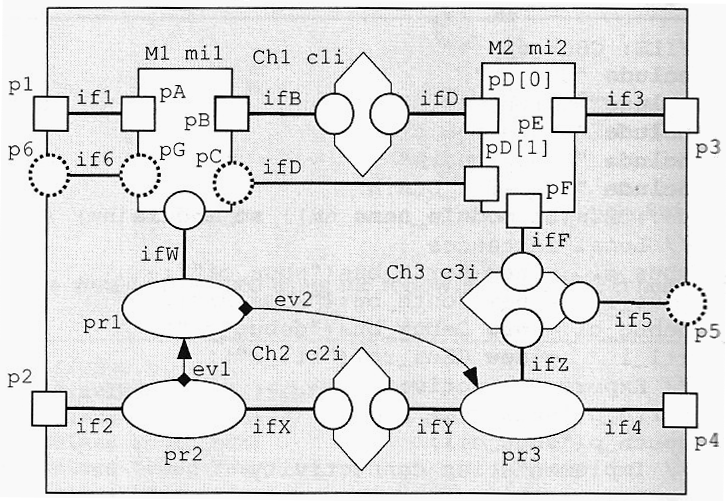
\includegraphics[width=0.6\textwidth]{lecture12/img/connections.png}
\end{figure}
{\scriptsize
\begin{itemize}
\item Rectangle: module
\item Square: port
\item Solid circle: implementing an interface
\item Dotted circle: export
\item Ellipse: process
\item Crystal: channel
\item Straight line: interface connection
\item Arrow: event dependency (from notifier process towards waiting process)
\end{itemize}
}
\end{frame}

\begin{frame}
\frametitle{Summary on connections}
\framesubtitle{Processes in the same module}

\begin{figure}
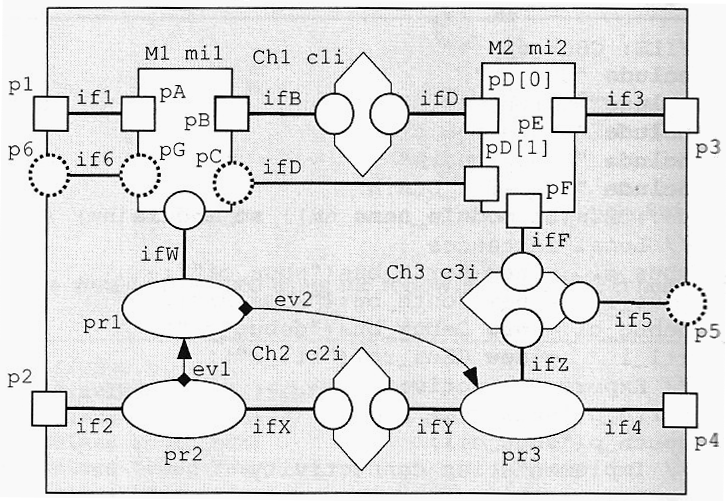
\includegraphics[width=0.6\textwidth]{lecture12/img/connections.png}
\end{figure}
{\scriptsize
\begin{enumerate}
\item A process may communicate with another process in the same module using a channel. For example, process \texttt{pr2} to \texttt{pr3} via interface \texttt{ifX} on channel \texttt{c2i}.
\item A process may communicate with another process in the same module using an event to synchronize exchanges of information through data variables instantiated at the module level (e.g., within
the module class definition). For example, process \texttt{pr2} to process \texttt{pr1} via event \texttt{ev1}.
\end{enumerate}
}
\end{frame}

\begin{frame}
\frametitle{Summary on connections}
\framesubtitle{Processes in different modules}

\begin{figure}
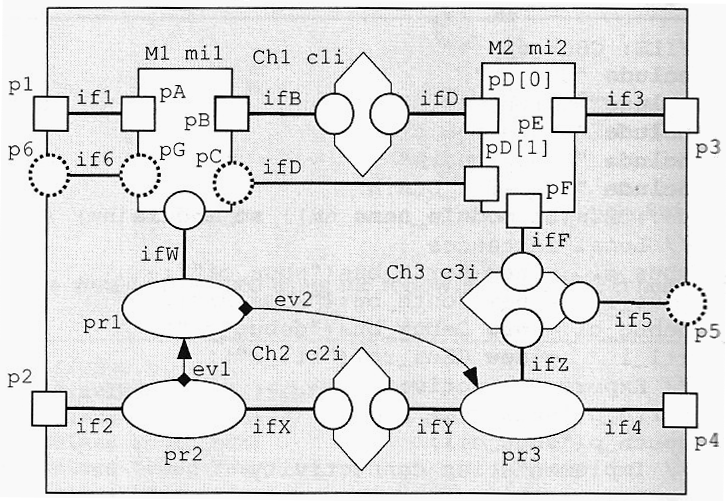
\includegraphics[width=0.6\textwidth]{lecture12/img/connections.png}
\end{figure}
{\scriptsize
\begin{enumerate}
\setcounter{enumi}{2}
\item A process may communicate with a process upwards in the design hierarchy using the interfaces accessed via \texttt{sc\_port<T>}. For example, process \texttt{pr3} via port \texttt{p4} using interface \texttt{if4}.
\item A process may communicate with processes in submodule instances via interfaces to channels connected to the submodule ports. For example, process \texttt{pr3} to module \texttt{mi2} via interface \texttt{ifZ} on channel \texttt{c3i}.
\end{enumerate}
}
\end{frame}

\begin{frame}
\frametitle{Summary on connections}
\framesubtitle{Generic ports}

\begin{figure}
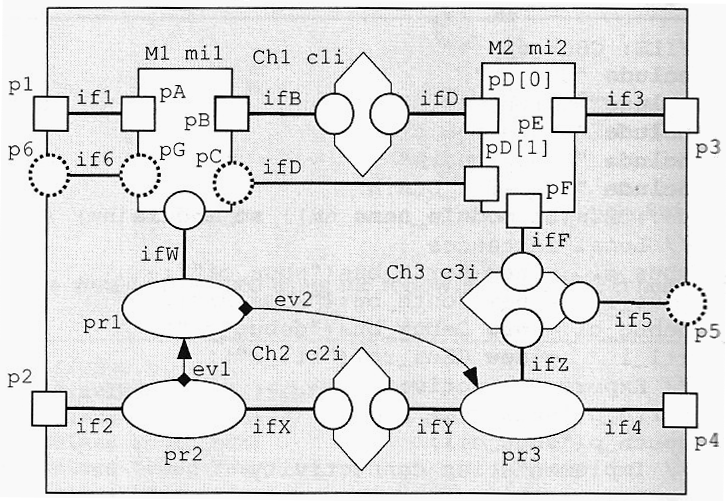
\includegraphics[width=0.6\textwidth]{lecture12/img/connections.png}
\end{figure}
{\scriptsize
\begin{enumerate}
\setcounter{enumi}{4}
\item An \texttt{sc\_port<T>} may connect directly to an \texttt{sc\_port<T>} of submodules. For example, port \texttt{p1} is connected to port \texttt{pA} of submodule \texttt{mi1}.
\item An \texttt{sc\_port<T>} may connect indirectly to a process by letting the process access the interface. This is just a process accessing a port described previously. For example, process \texttt{pr1} communicates with submodule \texttt{mi1} through interface \texttt{ifW}.
\item An \texttt{sc\_port<T,N>} array may be used to create multiple ports using the same interface. For example, \texttt{pD[0]} and \texttt{pD[1]} of submodule \texttt{mi2}.
\end{enumerate}
}
\end{frame}

\begin{frame}
\frametitle{Summary on connections}
\framesubtitle{Exports}

\begin{figure}
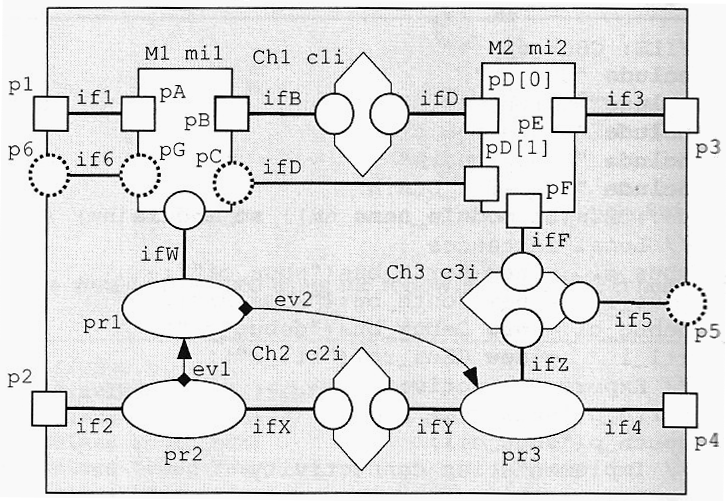
\includegraphics[width=0.6\textwidth]{lecture12/img/connections.png}
\end{figure}
{\scriptsize
\begin{enumerate}
\setcounter{enumi}{7}
\item An \texttt{sc\_export<T>} may connect to another \texttt{sc\_export<T>} via interfaces to local channels. For example, port \texttt{p5} to channel \texttt{c3i} using interface \texttt{if5}.
\item An \texttt{sc\_export<T>} may connect directly to an \texttt{sc\_export<T>} of a submodule. For example, port \texttt{p6} is directly connected to port \texttt{pG} of submodule \texttt{mi1}.
\end{enumerate}
}
\end{frame}